\chapter{Architecture Technique et Stratégie de Versioning}

\section{Fondements Théoriques de la Business Intelligence (BI)}
La Business Intelligence (BI) désigne l'ensemble des technologies et processus permettant de transformer des données brutes en informations exploitables pour la prise de décision. Le cycle de vie de la donnée dans notre projet suit les étapes classiques :
\begin{enumerate}
    \item \textbf{Collecte :} Extraction depuis les fichiers sources (CSV).
    \item \textbf{Intégration (ETL) :} Nettoyage et transformation pour assurer la qualité.
    \item \textbf{Stockage :} Organisation dans un modèle dimensionnel optimisé (Data Warehouse/Data Mart).
    \item \textbf{Analyse :} Création de mesures calculées (DAX).
    \item \textbf{Restitution :} Visualisation interactive pour les décideurs RH.
\end{enumerate}

\section{Choix de la Stack Technique et Justification}
Le choix s'est porté sur l'écosystème \textbf{Microsoft Power BI} pour plusieurs raisons stratégiques :
\begin{itemize}
    \item \textbf{Puissance du moteur VertiPaq :} Compression colonnaire permettant des performances exceptionnelles en mémoire.
    \item \textbf{Flexibilité de Power Query :} Langage M puissant pour les transformations complexes.
    \item \textbf{Richesse du DAX :} Capacité à modéliser des indicateurs métiers complexes (Time Intelligence, calculs de contexte).
    \item \textbf{Intégration :} Facilité de déploiement et de partage au sein de l'organisation.
\end{itemize}

\section{Architecture Conceptuelle de la Solution}
Pour assurer la robustesse et la maintenabilité, nous avons adopté une \textbf{architecture modulaire} en séparant les responsabilités dans trois fichiers Power BI distincts :

\begin{enumerate}
    \item \textbf{etl\_HR.pbix :} Dédié exclusivement à la connexion aux sources et aux transformations lourdes (M language).
    \item \textbf{dim\_HR.pbix :} Contient le modèle de données final (Star Schema), les relations et les colonnes calculées de base.
    \item \textbf{dax\_HR.pbix :} Focalisé sur la création des mesures analytiques et la conception graphique des rapports.
\end{enumerate}

\begin{figure}[h]
    \centering
    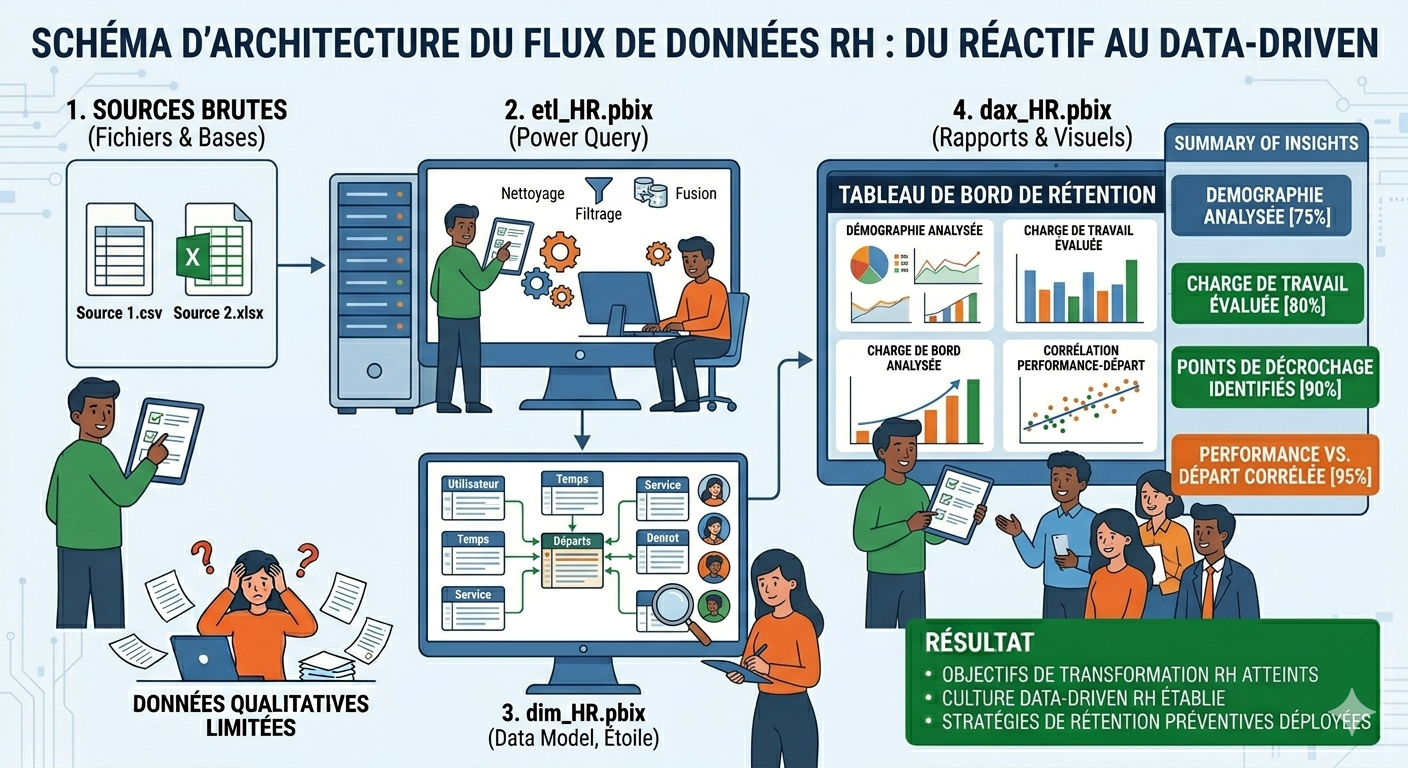
\includegraphics[width=0.8\textwidth]{figures/fig2_1_architecture.png.png}
    \caption{Flux de données et architecture modulaire}
    \label{fig:architecture}
\end{figure}

\section{Stratégie de Versioning et Git Workflow}
Le développement collaboratif a été orchestré via Git, permettant à chaque membre de travailler sur son axe de spécialisation sans interférer avec les autres :

\begin{itemize}
    \item \textbf{main :} Branche stable contenant la version de production validée.
    \item \textbf{feature/etl-pipeline :} Développement des flux M et nettoyage des sources.
    \item \textbf{feature/data-modeling :} Structuration des tables de faits et dimensions.
    \item \textbf{feature/kpi-logic :} Implémentation des formules DAX complexes.
    \item \textbf{feature/dashboard-design :} Travail sur l'ergonomie et les visuels.
\end{itemize}

Cette approche garantit une traçabilité complète des modifications et facilite l'intégration continue des nouveaux indicateurs.
